\section{Data Preprocessing}\label{data_preprocessing}

Data preprocessing is a vital step in the data mining process, particularly in the context of deep learning for image classification. This step involves techniques such as image augmentation, affine transformations, and resizing, which are essential for enhancing model performance. For this project, preprocessing is applied to the provided dataset (dataset\_19) to ensure it is suitable for the brain tumor classification task. The specific steps involved in the preprocessing of this dataset are outlined below.

\subsection{Dataset}\label{dataset_given}

The dataset, referred to as dataset\_19, comprises a folder containing four subfolders, each representing a different class of brain tumors. Each subfolder includes 120 MRI images of varying image sizes. The dataset distribution is illustrated in Figure \ref{fig:data_distribution}.

\begin{figure}[H]
  \begin{center}
    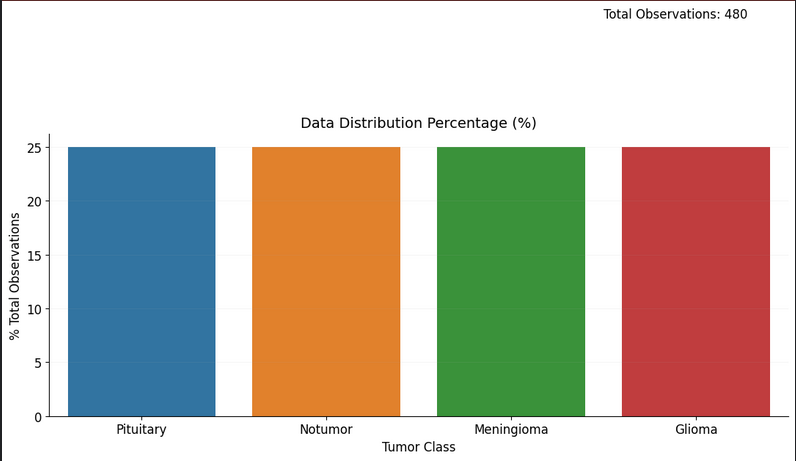
\includegraphics[width=0.95\textwidth]{Exploration/data_distribution.png}
  \end{center}
  \caption{Distribution of images in dataset\_19.}\label{fig:data_distribution}
\end{figure}

\subsection{Image Sizes}\label{image_sizes}
The overall average size of the images is approximately $[453.36, 450.83]$ pixels. The smallest image size is $(198, 150)$ pixels, and the largest image size is $(1075, 890)$ pixels. The mean, median, and mode sizes across the dataset are consistent at $[512, 512]$ pixels, suggesting a central tendency around these dimensions.


\begin{figure}[H]
  \begin{center}
    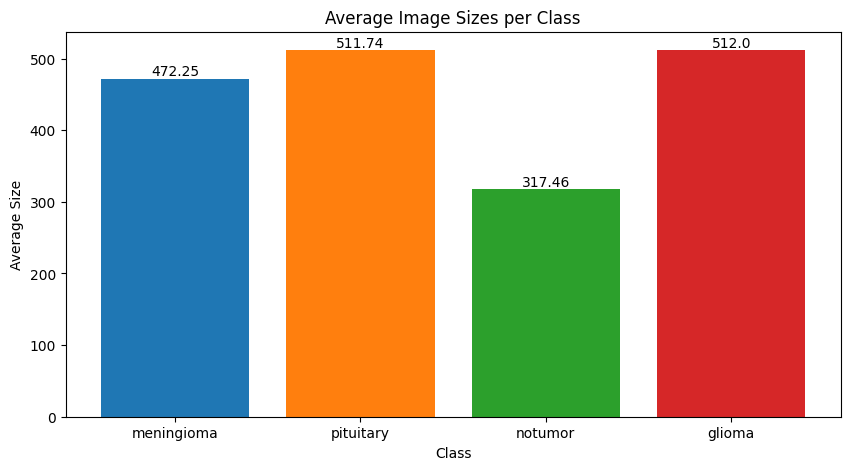
\includegraphics[width=0.95\textwidth]{Exploration/data_sizes.png}
  \end{center}
  \caption{Distribution of brain image sizes in dataset\_19.}\label{fig:data_sizes}
\end{figure}

\begin{longtable}{|l|c|c|}
\caption{Overall Statistics of Brain Image Sizes}\\
\hline
\textbf{Statistic} & \textbf{X} & \textbf{Y} \\
\hline
\endfirsthead
\hline
\textbf{Statistic} & \textbf{X} & \textbf{Y} \\
\hline
\endhead
\hline
\endfoot
\endlastfoot
\textbf{Mean Size} & 453.3625 & 450.83125 \\
\hline
\textbf{Median Size} & 512 & 512 \\
\hline
\textbf{Mode Size} & 512 & 512 \\
\hline
\textbf{Standard Deviation of Size} & 124.1067 & 131.5980 \\
\hline
\textbf{Variance of Size} & 15402.4644 & 17318.0236 \\
\hline
\textbf{Smallest Size} & 198 & 150 \\
\hline
\textbf{Largest Size} & 1075 & 890 \\
\hline
\end{longtable}

\vspace{1cm}

\begin{longtable}{|l|c|c|c|c|}
\caption{Class-Specific Statistics of Brain Image Sizes}\\
\hline
\textbf{Statistic} & \textbf{Meningioma} & \textbf{Pituitary} & \textbf{Notumor} & \textbf{Glioma} \\
\hline
\endfirsthead
\hline
\textbf{Statistic} & \textbf{Meningioma} & \textbf{Pituitary} & \textbf{Notumor} & \textbf{Glioma} \\
\hline
\endhead
\hline
\endfoot
\endlastfoot
\textbf{Mean Size (X)} & 472.25 & 511.7417 & 317.4583 & 512 \\
\hline
\textbf{Mean Size (Y)} & 466.4083 & 510.5417 & 314.3750 & 512 \\
\hline
\textbf{Median Size (X)} & 512 & 512 & 236 & 512 \\
\hline
\textbf{Median Size (Y)} & 512 & 512 & 236 & 512 \\
\hline
\textbf{Mode Size (X)} & 512 & 512 & 236 & 512 \\
\hline
\textbf{Mode Size (Y)} & 512 & 512 & 236 & 512 \\
\hline
\textbf{Standard Deviation of Size (X)} & 100.7078 & 43.5696 & 154.5843 & 0 \\
\hline
\textbf{Standard Deviation of Size (Y)} & 108.4743 & 30.7834 & 174.3213 & 0 \\
\hline
\textbf{Variance of Size (X)} & 10142.0708 & 1898.3083 & 23896.3149 & 0 \\
\hline
\textbf{Variance of Size (Y)} & 11766.6749 & 947.6149 & 30387.9010 & 0 \\
\hline
\textbf{Smallest Size (X)} & 223 & 256 & 198 & 512 \\
\hline
\textbf{Smallest Size (Y)} & 200 & 256 & 150 & 512 \\
\hline
\textbf{Largest Size (X)} & 650 & 903 & 1075 & 512 \\
\hline
\textbf{Largest Size (Y)} & 591 & 721 & 890 & 512 \\
\hline
\end{longtable}

Class-specific statistics show variation in image sizes:
\begin{itemize}
    \item \textbf{Meningioma}: Sizes range from $(223, 200)$ to $(650, 591)$ pixels, with a mean size of approximately $[472.25, 466.41]$ pixels.
    \item \textbf{Pituitary}: Sizes range from $(256, 256)$ to $(903, 721)$ pixels, with a mean size of approximately $[511.74, 510.54]$ pixels.
    \item \textbf{Notumor}: Sizes range from $(198, 150)$ to $(1075, 890)$ pixels, with a mean size of approximately $[317.46, 314.38]$ pixels.
    \item \textbf{Glioma}: All images are consistently sized at $[512, 512]$ pixels.
\end{itemize}

The variability in image sizes across different classes highlights the importance of size normalization during the preprocessing phase. For instance, while the `glioma` class images are uniformly sized, other classes exhibit significant variation, which could introduce biases or inconsistencies in the training process if not properly addressed.

Proper preprocessing, including size normalization, is vital for several reasons:
\begin{itemize}
    \item \textbf{Uniform Input Size}: Neural networks require inputs of a fixed size. Without resizing, it would be impossible to batch process the images.
    \item \textbf{Consistent Feature Representation}: Ensuring all images are of the same size ensures that features are represented consistently across the dataset, which aids in better model learning.
    \item \textbf{Reduction of Computational Load}: Smaller, consistent image sizes can significantly reduce the computational load and memory requirements, making training more efficient.
    \item \textbf{Enhanced Model Performance}: Properly preprocessed images can lead to improved model convergence and accuracy, as the network can learn from a standardized set of inputs.
\end{itemize}

In conclusion, the preprocessing step of resizing images to a uniform dimension is an essential consideration in developing a robust and efficient deep learning model for brain tumor classification. It not only facilitates smooth training but also contributes to the overall performance and generalization capability of the model.

\subsection{Data Splitting and Augmentation}\label{data_split_augmentation}
To prepare the dataset for the classification task, it is preprocessed and subsequently divided into training and validation sets, with the training set comprising 80\% of the data and the validation set 20\%. This split is shown in Figure \ref{fig:data_split}. The training set is used to train the model, while the validation set is used to evaluate its performance.

\begin{figure}[H]
  \begin{center}
    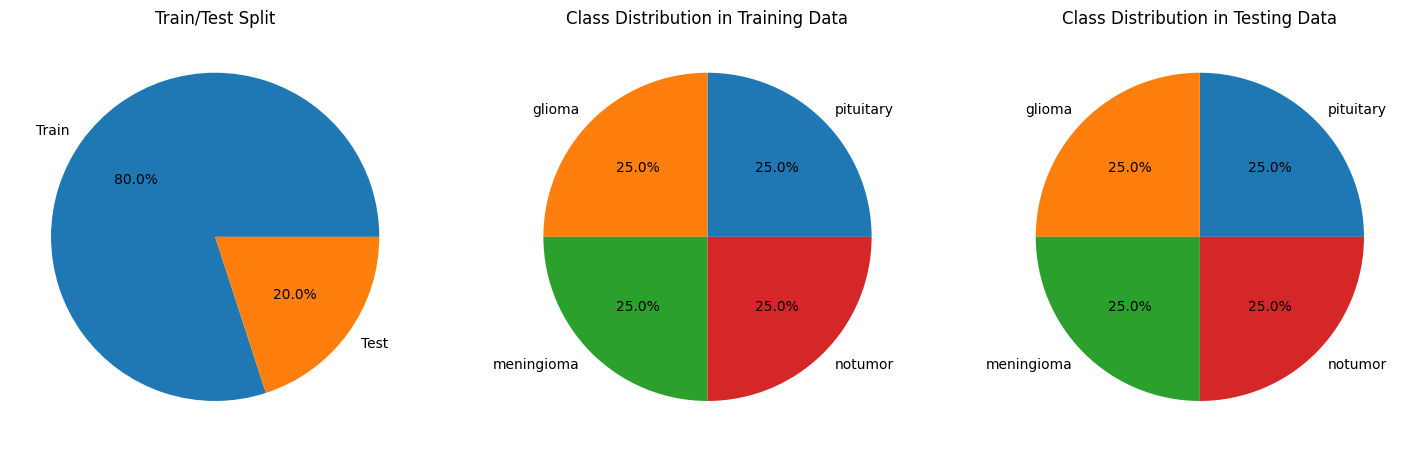
\includegraphics[width=0.95\textwidth]{Exploration/data_split.png}
  \end{center}
  \caption{Splitting the dataset into training and validation sets.}\label{fig:data_split}
\end{figure}

Image preprocessing is essential to enable models to focus on the region of interest, namely the brain, while reducing background noise and irrelevant features. This process involves converting images to grayscale, applying Gaussian blur, and performing thresholding and morphological operations to refine image quality. By cropping around the largest contour, which is likely the brain, this step highlights critical anatomical features and enhances model generalization, ultimately leading to more accurate tumor classification.

\begin{figure}[H]
  \begin{center}
    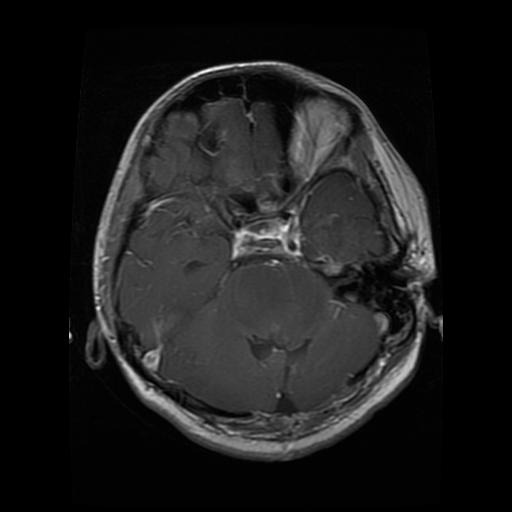
\includegraphics[width=0.3\textwidth]{Exploration/Te-gl_0010.jpg}
    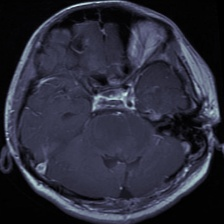
\includegraphics[width=0.3\textwidth]{Exploration/Te-gl_0010_preprocessed.jpg}
  \end{center}
  \caption{Cropping the MRI image along its contour.}\label{fig:image_cropping}
\end{figure}

Image augmentation is then performed using the \texttt{ImageDataGenerator} class from the Keras library. This technique artificially increases the dataset size by applying various transformations to the images, thus improving model performance by providing more training data. The \texttt{ImageDataGenerator} class offers several parameters for image augmentation.

The preprocessing pipeline involves initially performing horizontal flips on the images, followed by random rotations. Each image is then normalized by dividing pixel values by 255. After these transformations, the dataset is split into training and validation sets as previously described.

\subsection{Summary and Justifications}

Given the relatively small size of dataset\_19 (480 images in total), data augmentation is crucial for enhancing the dataset's variability and improving the model's generalization capabilities. Flipping images horizontally is justified based on the anatomical symmetry of the brain's hemispheres, allowing for effective augmentation without misrepresenting tumor locations \cite{nalepa_data_2019}. This technique increases the diversity of the training data, which is particularly important given the limited size of the dataset compared to larger datasets, such as those used in the BraTS competition.

Similarly, random rotations are applied since brain images can be rotated in various directions, further increasing the dataset's variability and aiding in model training. The augmentation strategies, including horizontal flipping and random rotations, are essential for compensating for the smaller dataset size by exposing the model to a wider variety of image orientations and perspectives. This approach helps create a more robust model capable of accurately classifying brain tumors despite the limited amount of original training data.

